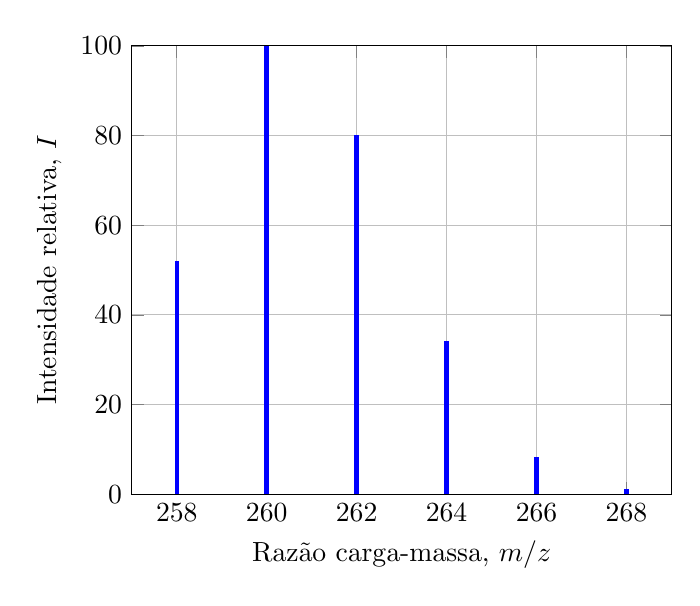
\begin{tikzpicture}
    \begin{axis}
        [
            grid = major,
            ylabel = {Intensidade relativa, $I$},
            xlabel = {Razão carga-massa, $m/z$},
            ymin = 0,
            ymax = 100,
        ]
    \addplot[blue, ultra thick, mark=none] coordinates
        {
            (258, 00)
            (258, 52.071171)
        };
    \addplot[blue, ultra thick, mark=none] coordinates
        {
            (260, 00)
            (260, 100.000000)
        };
    \addplot[blue, ultra thick, mark=none] coordinates
        {
            (262, 00)
            (262, 80.030369)
        };
    \addplot[blue, ultra thick, mark=none] coordinates
        {
            (264, 00)
            (264, 34.167975)
        };
    \addplot[blue, ultra thick, mark=none] coordinates
        {
            (266, 00)
            (266, 8.209707)
        };
    \addplot[blue, ultra thick, mark=none] coordinates
        {
            (268, 00)
            (268, 1.053385)
        };
    \end{axis}
\end{tikzpicture}
